\documentclass[letterpaper,10pt, draftclsnofoot,onecolumn]{IEEEtran}
\usepackage[top=0.75in, bottom=0.75in, left=0.75in, right=0.75in]{geometry}

\usepackage{amsmath}
\usepackage{amssymb,amsfonts,textcomp}
\usepackage{color}
\usepackage{array}
\usepackage{supertabular}
\usepackage{hhline}
\usepackage{hyperref}
\usepackage{float}
\usepackage{type1cm}
\usepackage[english]{babel}
\hypersetup{pdftex, colorlinks=true, linkcolor=black, citecolor=blue, filecolor=black, urlcolor=black, pdftitle=SYSTEMS AND SOFTWARE REQUIREMENTS SPECIFICATION (SSRS) TEMPLATE}
\usepackage[pdftex]{graphicx}
% Outline numbering
%\renewcommand{\thesection}{\arabic{section}}
%\renewcommand{\thesubsection}{\thesection.\arabic{subsection}}
%\renewcommand{\thesubsubsection}{\thesubsection.\arabic{subsubsection}}


\makeatletter
\newcommand\arraybslash{\let\\\@arraycr}
\makeatother
% Page layout (geometry)
\usepackage{geometry}
\geometry{textheight=8.5in, textwidth=6in}
% Footnote rule
\setlength{\skip\footins}{0.0469in}


% footnotes configuration
\makeatletter
\renewcommand\thefootnote{\arabic{footnote}}
\makeatother
\title {Design Document}
\author{Zixuan Feng
	   Jason Ye
	   David Corbelli }
\date{October, 2016}
\begin{document}

\begin{flushleft}

   
        \Huge\textbf{Design Document}\\
        \vspace{1.6cm}
        \large Sponsor \\
      	\LARGE\textbf {Oregon State Department of Education}\\
        \vspace{1.2cm}
        \LARGE\textbf {Prepared by Capstone 41}\\
        \large David Corbelli, Jason Ye, Zixuan Feng
        \vspace{1.9cm}
\end{flushleft}
        \newpage
    	\selectlanguage{english}\color{black}\normalsize\noindent{\textbf{Abstract:} The application and website for Oregon science is a guide for middle school and high school level students to learn about health science careers. 
        Between an application and website, the service shall provide information as exploration tool for students looking for future careers in health science. 
        Due to the many fields under the classification of health and science, it may be difficult for a student beginning to take an interest in the subject to find the proper path they're looking for.
        As a development team we will focus on developing an exploratory website and then develop corresponding applications for Android OS. 
        Through our platform, students will explore pathways and careers in health and science.}
        
       
        

%%%%%%%%%%%%%%%%%%%%%%%%%%%Heading part%%%%%%%%%%%%%%%%%%%%%%%%%%




\vspace{-1.5cm}
\setcounter{tocdepth}{9}
\renewcommand\contentsname{}


\clearpage{\selectlanguage{english}\color{black}
\tableofcontents

\clearpage{\selectlanguage{english}\color{black}

\section[Overview]{\selectlanguage{english}\color{black}
Overview}

\subsection{Scope}{\selectlanguage{english}\noindent\color{black}
This project consists of creating a website and mobile application that will provide accurate and updated information based upon information from the Oregon Department of Education. 
Modules of the website and application include information pertaining to career pathways, industry events, and administration tools.

\subsection{Purpose}{\selectlanguage{english}\noindent\color{black}
This document is intended to detail the implementation of each component pertaining to the project. It also describes the components and steps of applying and creating of the technologies.
Decisions discussed within this document concern relational databases, Google Analytics and Android platform, written by Jason Ye,  MySQL, testing options, and Android Studio, written by Zixuan Feng, and hybrid application development,  Twitter bootstrap, and template paged generation, written by David Corbelli.
We have conducted research on these technologies and they have been selected as the best-fit technologies for this project. 

\subsection{Intended Audience}{\selectlanguage{english}\noindent\color{black}
The intended audience of this project is aimed towards high school students and their parents. Students at this level begin to choose their future career paths and to some it is still unclear how to take steps towards these goals and what requirements they need to fulfill. 
The website and application developed through this project will become a user-friendly means to fill this gap. 

\subsection{Timeline}{\selectlanguage{english}\noindent\color{black}
The development of this project will occur in three major phases. 
The first includes designing the web page layout, styling, navigation and back-end database setup. 
The next phase entails the implementation of these design choices, primarily, the coding of HTML pages and the PHP scripts to read from the database. 
The third and final phase is the implementation of the mobile site and Android application.
The latter of these tasks is to be heavily influenced by the former, as such their development is grouped.
\begin{figure}[H]
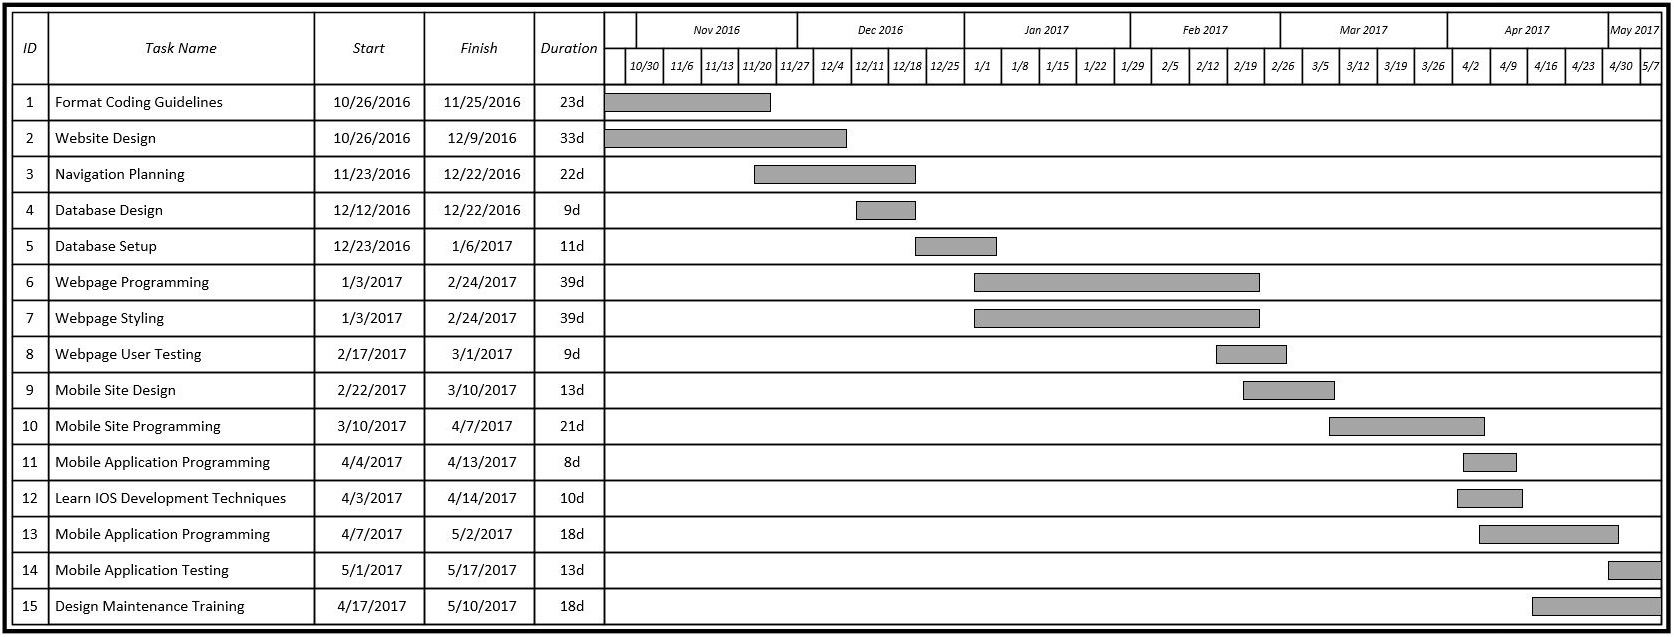
\includegraphics[scale=0.5]{GANTTv2.jpeg}
\end{figure}


\clearpage{\selectlanguage{english}\color{black}
\section[Definitions]{\selectlanguage{english}\color{black}
Definitiosn}

\selectlanguage{english}\noindent\color{black}\textbf{Application Programming Interface:} A set of routines, protocols and tools for building software applications. 

\selectlanguage{english}\noindent\color{black}\textbf{AVD Manager:} Android Virtual Device(AVD) will performs as different Android devices.

\selectlanguage{english}\noindent\color{black}\textbf{Bulk Copy Program:} Program that copies data between an instance of MicrosoftSQL server and a data file in a user-specified format.}

\selectlanguage{english}\noindent\color{black}\textbf{Cascading Style Sheets (CSS):} The primary language used for remodeling the visual presentation of a website

\selectlanguage{english}\noindent\color{black}\textbf{Database:} A structured set of data held in a computer, especially one that is accessible in various ways.}

\selectlanguage{english}\noindent\color{black}\textbf{Debugger:} A computer program that assists in the detection and correction of errors in computer programs.

\selectlanguage{english}\noindent\color{black}\textbf{Emulator:} A hardware or software that enables one computer system to behave like another computer system.  

\selectlanguage{english}\noindent\color{black}\textbf{ER diagram:} Entity-relationship model means related things in the database in specific domain. 

\selectlanguage{english}\noindent\color{black}\textbf{HyperText Markup Language (HTML):} The standard programming language used for creating web pages

\selectlanguage{english}\noindent\color{black}\textbf{Integrated Development Environment:} A software application that provides comprehensive facilities to computer programmers for software development.

\selectlanguage{english}\noindent\color{black}\textbf{Library:} A package of pre-written code that may be called upon for a variety of purposes.

\selectlanguage{english}\noindent\color{black}\textbf{Metadata:} A set of data that describes and gives information about the HTML document. }

\selectlanguage{english}\noindent\color{black}\textbf{Mysqldump:} Mysqldump usually performs intelligent reinforcements, creating a set of SQl proclamations that could be executed to recreate the first database object definition and table information.

\selectlanguage{english}\noindent\color{black}\textbf{Operating System:} The software that supports a computer's or mobile device's basic functions.

\selectlanguage{english}\noindent\color{black}\textbf{PHP:} A scripting language used to instruct operations performed by the server

\selectlanguage{english}\noindent\color{black}\textbf{Plugin:} A software component that adds a specific feature to an existing computer program. 

\selectlanguage{english}\noindent\color{black}\textbf{Relational Database Management System:} The various software systems used to maintain relational databases.}

\selectlanguage{english}\noindent\color{black}\textbf{SDK:} Software Development Kit. 

\selectlanguage{english}\noindent\color{black}\textbf{Source Code:} Any collection of computer instructions, written in programming language, as a ordinary text.

\selectlanguage{english}\noindent\color{black}\textbf{Statistics:} A collections of numerical data in large quantities. }

\selectlanguage{english}\noindent\color{black}\textbf{Structured Query Languages:} A programming language that is used to communicate with a database.}

\selectlanguage{english}\noindent\color{black}\textbf{Software Framework:} An abstraction of generic functionality allowing for selective change in functionality by the use of additional code

\selectlanguage{english}\noindent\color{black}\textbf{UI Design:} UI Design means user interface design, such as computers, applications, and websites.

\clearpage{\selectlanguage{english}\color{black}
\section[Design Descriptions]{\selectlanguage{english}\color{black}
Design Descriptions}
\subsection[Database Type]{\selectlanguage{english}\noindent\color{black}
Database Type}
{\selectlanguage{english}\noindent\color{black}
The most important aspect of our project is to have a place to store a large amount of information.
In addition, the ability to edit the information by adding, deleting, and updating is crucial for an informative website such as our project. 
A technology such as a database to keep a collection of data that can easily be accessed and managed is necessary to have.
Our project is to create an informative website and application, and a database is the most appropriate technology to use. 
\\ \\
\noindent Within the different types of database, the most common of all is the relational databases.
In this field, we would be implementing the data in a relational database and store them in various data tables. 
Simply a relational database system contains one or more objects are called tables \cite{website2}. 
Every table will be uniquely identified by their names, and each name is comprised of columns and rows.
Supposed we have information about a specific health science career. 
In a table, the name would be the name of the career, the column contain the column name, data type, and other attributes for the column, and rows contain the records or data for the column such its degree of completion or GPA requirement. 
Each table must follow a certain integrity rules to ensure that the data are always accessible. 
For the rows in a table, they should all be distinct. 
Duplicated rows can be lead to possible selection problems. 
Fortunately, database system allows developer to specify that duplicated rows are not allowed. 
\\	\\
\noindent In the case of relational database, there is a Relational Database Management System (RDBMS) which handles the way data is being stored, maintained, and retrieved \cite{website2}. 
In addition, we would be using RDBMS, because it is the best option for the storage of data in databases used for educational information such as our project. 
RDBMS also provide the usage of Structured Query Languages (SQL) to communicate with a database. 
SQL is a language designed to be used with relational databases.
The implementation of SQL tends to be standard and is used by all RDBMSs.
In addition, SQL is the technique to retrieve data from a database, or update data on a database. 
Before accessing the databases, all of the data must be implemented in tables. 
To input a large amount of data into the database, we would be using Bulk Copy Program (BCP). BCP is a command line tool within the SQL server that export text file into SQL server. 
With that ability, any size of file can be imported into our server automatically. 
After all of the information is completely stored, we would be using SQL to access the large amount of data directly from the database. 
From that point on, we would be able to deliver valuable contents onto the website and phone app for our audience to view. 
}

\subsection[Database Hosting]{\selectlanguage{english}\noindent\color{black}
Database Hosting}
\noindent Due to our mission, we are going to developed a website, and the main function of the website is going to exhibit information to users. To make sure the stabilization of database is our priority goal, according to the book “Building Your Next Big Thing with Google Cloud Platform”\cite{book7},Google company will help the user to maintain the server. Since we will make a notebook for future database management, and we cannot make sure the future website manager are experienced with web development,  Google Cloud SQL is an easy tool to manage in the future. What is more, Google Cloud SQL always store the data in the cloud, it is easy and safe for the future database managers. According to the Google Cloud SQL, Google company store the data in different data centers at same time, which gives user a safer environment. Currently, The Google Cloud SQL has compatible with JAVA and Python, which is same as the MySQL as for programming language, we are all familiar with python and MYSQL, so this tool fits our language skill and it could allow the programmer use the MysqlIDump import the database. Due to the budget, since our client is government, we need to control our budget and help the government to save money. As we compared, Google Cloud SQL is one of the cheapest tool to use. 
\\ \\
\noindent However, there are two disadvantages of Google Cloud SQL, first is GCS only could provide 100GB memory. Considering our website mission, 100 GB is enough for our website. And  Google Cloud SQL limits the search speed as 16MB/Seconds, but it could also fit our websites’ data.
\\ \\
\noindent As for creating database in the Google Cloud Sql, firstly, we need to figure how many tables we need to create. Based on our website and current data we gathered, at least 6 tables we need to create at first: user accounts, current events lessons, career pathways, contents of health careers, education tool box and career resource. Besides of these tables, we also need to create an ER diagram for our database, which is helpful for us to create table, since it will show us the clear relationship of each table. After creating the table, we just need to use MySQL query to check and calculate all the information in each table.
\subsection[Twitter Bootstrap]{\selectlanguage{english}\noindent\color{black}
Twitter Bootstrap}
{\selectlanguage{english}\noindent\color{black}
One of the most noticeable features of a website is its styling. 
Rather than writing our own CSS document to customize our page layout, fonts, and navigation bars, we are able to use an open-source styling framework. 
Utilizing a publicly available styling framework will allow us to achieve a marginally similar if not greater level visual presentation than we could manage ourselves, while allowing for the reallocation of time towards other essential features of the website. 
Evaluating several frameworks upon criteria including usability, documentation, compatibility, and visual output, Twitter's Bootstrap is the decidedly optimal implementation
\\ \\
Bootstrap, the styling framework developed and utilized by Twitter's main website, is reliant upon the specification of HTML class tags to determine how styling should be applied to specific page components. 
This allows for individual customization of each element. 
Bootstrap also incorporates a grid system to allow for quick changes in layout, while other options also include custom fonts, colors, and pre-built navigation bars. 
For increased responsiveness, the navbars and page components may be collapsed to better fit the window size of desktop and mobile devices.  
\\ \\
The implementation requirements for Bootstrap are simple. 
The Bootstrap package must be either downloaded as a local package to be stored server-side, or linked to the online GitHub hosted project library. Both of these options are equally as functional for out project, however, the server-side implementation allows for greater fidelity should connectivity to the GitHub library suffer.
This decision may also benefit load-time issues associated with loading in page information from a nonnative source. There exists thorough documentation, both first-party and third-party, for webpage design templates and usable class tags.
Basing our own styling upon pre-existing templates provides a starting point before delving further into individual design choices tailored for this particular website.
However, before determining which template to implement as a baseline, a prototype page layout for each page will be drafted to visualize different styles and pagebody organization. 
Once design planning has concluded, a template webpage containing the navigation bar, header, and footer will be drafted as the standard frame by utilization of bootstrap templates and class tag selection, while the body of each page is to be developed individually or loaded in through a combination of PHP and Javascript depending upon the content type.
\\ \\
As the website is directed towards middle and high school students, a design format familiar to the target audiences will allow the users more comfort as they use the site. 
Aside from assisting with the functional organization of our webpages, open-source pre-developed themes will give the website a modern feel with features including background images and dynamic page content.
\\ \\
In order to save time in developing between both the desktop and mobile versions of the site, Bootstrap has been chosen to provide scalable navbars and borders in order to maintain consistency across platforms. Utilizing these specific classes will minimize the discrepancies between the separate coding implementations and will also assist in upholding a visual standard across differences in devices and screen sizes. 
\\ \\
In implementation. Bootstrap serves to improve this website's potential in terms of visual output and time allocation.
}

\subsection[Templated page Generation]{\selectlanguage{english}\noindent\color{black}
Webpage Generation}
{\selectlanguage{english}\noindent\color{black}
Templated page generation is another practice that allows for efficient allocation of development time. 
Each web page comes with a variety of requirements; navigation bars, headers, footers, and CSS styling associated with each as well as the main page body are all pieces of redundant code to be used across each page.
Rather than re-coding the CSS specifications for each page allowing for marginally greater control over each page's appearance, creating a single coded framework to act as the standardized website page style will save time and increase consistency across all pages. 
Considering the implementation choice to utilize Twitter's Bootstrap, consistency between styling class tags will be essential due to the sheer variance in the framework's styling.
\\ \\
The implementation will require several steps. 
First, the appearance and organization of the page must be drafted and improved upon until a finalized version of each page can be visualized. 
With this implementation it is also necessary to ensure that the layout of each page is similar enough or standardized to the point that no page styling may conflict with organization of another.
Second, the basic HTML code containing the necessary elements for all pages, including the header, footer, navigation bars, and primary page body sections will be coded with empty class tags. 
The main page body must be developed separately after the template's completion and the displayed information will vary based upon the page’s purpose within the site. 
With the infrastructure of each page in place, the next step is to reference the drafted site styling with the available styling tags within the Bootstrap library. 
The most simple option is to identify an existing Bootstrap template and to fill in the necessary HTML code to fit our site. 
This operation must be done for each page component to ensure the majority of the page is consistently styled with Bootstrap.
\\ \\
The adoption of this page generation strategy should serve to reduce the amount of coding time required by each page. After the basic HTML or PHP files for each web page are created using the template, the remaining section of page body must be filled in with the required code. These sections will also require styling choices, while not implemented using a template, must require conformance to similar styles amongst other the pages. 
\\ \\
Once the procedure has been implemented for the desktop site, a similar process must be undertaken for the mobile site design and development. As most of the styles available through Bootstrap are capable of scaling to screen size, many of the necessary page components including headers, footers, and the navigation bar are able to collapse to versions suitable for mobile devices, requiring no change in implementation. For other page elements it may be necessary to identify different class types from the desktop site for optimal viewing through mobile browsers.
\\ \\
The creation of web pages based off of a devised template will serve to uphold the consistency of the website and application visuals and save time in development.

}

\subsection[Web Statistics]{\selectlanguage{english}\noindent\color{black}
Web Statistics}
{\selectlanguage{english}\noindent\color{black}
For the purpose of maintaining the website, we needed a service that will analyze the website statistics for trends and success level.
Alternatively, we need a visualization tool that can display the data in a meaningful way for client and programmer to see.
It is important to have a log file that measure the behavior of visitors and track details, because it is useful for market research. 
Also, it is crucial for us to know what is needed to be evaluated on the site’s content to ensure that visitors are finding what they want.
The best measurement, collection and reporting of web data would be Google Analytic. 
\\	\\
\noindent Google Analytics lets us analyze user behavior on the website to improve user experience and ensure the success of our project \cite{website1}. 
Before beginning to analyze the website statistics, it is necessary to create an analytics account. 
After an account is made, a number of instructions will be given for setting up the Google Analytics.
The first step is to have Google verifies the website.
After verification, a tracking code will be provided for identification. 
The tracking code will identify and collect data from the website. 
This decision must be followed in order for Google to know when the site is visited. 
In addition, these scripts of coding must be installed on every page on the website.
The coding varies depend on the type of website. Because our website will be built on HTML files, we will add the tracking code inside the metadata container. 
After a successful implementation of the tracking code, the site is ready to show data statics on Google Analytics.
With its data, we can start learning about our website traffic. 
A detailed report will be shown each time we connect to Google Analytics.
\\	\\
\noindent Google Analytics provide different useful reports for analysis.
One of the reports Google Analytics provide is an audience report. 
Audience reports inform about visitors who show interest in our website. 
These visitors are our main customer, and we would find detailed report for their demographics, interests and location. 
Similar to audience reports, acquisition reports would inform data about what drove visitors to our site.
In this report, our data show which channels or promotions lead visitor to our site.
With that data, we could increase our potential growth of audience by advertising the site on specific social networks. 
In addition to analyzing visitor's data, Google Analytics offers a behavior reports which reveals what our visitors do on the website.
The general overview of the report provides the traffic of page views, average amount of time users spend viewing a page, percentage of single page visits, and percentage of user who exit from a page. 
These reports can help us determine if visitors are finding what they are looking for on the website.  
}

\subsection[Testing]{\selectlanguage{english}\noindent\color{black}
Testing}

\noindent As for our project testing, we are going to use all these three testing method to test our website and application: tree testing, click testing and remote usability testing. 
\\ \\
\noindent For tree testing, According to the article “Solving Site Navigation Issues with Tree Testing” \cite{article4}which is the first testing method for web development, since all the functions of website are based on the tree relations. As for steps of tree testing: firstly, we need to choose a mission task, for example we want to search information about health career, at first we need to test “sign in and register” to make sure user could use the research function as a website user. And we could test whether we could use the research function, so we could type some information in the search container, and then check the result whether is related to “health career”. Based on the result, click any of the research result to check whether it is clickable and it is related to “health career” information. After done with this task, we could choose another task to test other functions of website until test all the functions.
\\ \\
\noindent For click Testing. as for another basic testing method is going to test all the website and application button whether is clickable, which includes navigation and functionality. According to the article “Getting The First Click Right” \cite{article5}Same as the tree testing, we need to focus on the “Where to”, “how to” and “Where is”. But we need to know the correct path of mission, and do the each “click” in orders, and record the time. At last, we need to conclude the entire click testing process whether it could go to correct destination through correct path.
\\ \\
\noindent Besides of these two testing method, we need to  use the “remote usability testing”. “Click testing” and “Tree testing” are all controlled by professional tester, like programmers, however no matter website or application, the main users are non-professional users, so we need to use the “remote usability testing” to let general users to test website and application. According to the website, “Unmoderated, Remote Usability Testing: Good or Evil?” \cite{article6}
Since general and new users do not know our website and application, they will only follow their general experience and computer knowledge to finish the mission, which could help developers to find bugs during normal using. As for the specific process, we could choose 10 tester and we do not want tester are related to computer science career. To make the tester efficient and effective, we could choose various age testers: 4 testers around 15 years old, 2 testers around 20 years old, 2 testers around 30 years old, and 2s tester around 10 years old. Since our range age users are from 10-30 years, so we could cover all these age testers. And setting up 3-5 different missions to ask user to finish, for example, “ search health career job and find a related result”. Considering the different missions, we should set the time limit, since  if the tester cannot finish it on time, which means the task is designed too complicated. As for the negative factors of remote usability testing, we should avoid these factors. First, we should not limit our tester’s time, we could just give them a time range to finish it instead of at some specific time. In this way, we could give tester a more flexible time to users. And then, to avoid some bad attitude of tester, we could give them tread to finish it. For instance, we could give them a 5 dollar gift card to finish the test. In this way, the gift card to increase tester’s engagement. Once they finish the test, and we think their test processes are finished carefully, we could give them a tread as appreciation.




{\selectlanguage{english}\noindent\color{black}

}

\subsection[Mobile OS Platform]{\selectlanguage{english}\noindent\color{black}
Mobile OS Platform}
{\selectlanguage{english}\noindent\color{black}
Besides providing a website, we are require to develop a mobile application on a mobile operating system platform.
The major platform requirement for the project is to create an application on an Android platform, which is an open source mobile system. 
Its massive user base offers the best technology framework in the Android community.
One of the best tool Android offers is Android Software Development Kit (SDK), 
which is a development tool to develop applications for Android platform. SDK are comprised of application programming interfaces (APIs).
Also, it provides many unique set of tools such as debugger, emulator, sample code, documentation, source code, and libraries for a wide range of usage.   
\\	\\
\noindent Because Android is an open source mobile operating system (OS), its source code can be taken and altered by anyone when released \cite{website3}. 
As its source code is widely available for people to change, many variants of the OS, adapted to different hardware platforms, are showing up. 
Its open nature has encouraged a large community of developers to use as a foundation for many projects.
Its driven projects deliver updates to older devices or add new features for advanced users.
\\	\\
\noindent Android platform is hosted by Google, there are many important players such as: IDE, documentation, and Google Play in the system. 
Before implementation, one’s first consideration of building an Android app is a right tool. Usually, a recommended tool such as the Integrated Development Environment (IDE) is used for app development.
To access Android’s IDE, one download the Eclipse IDE, which is a Java-based open source platform, and Android developer tools plugin. 
The next tool is documentation; it is a problem that most developer faces when working on Android app.
Because the apps have to be installed on top of the Android OS, developer must know which Application Program Interface (API), which is a set of protocols and tools for building software applications, they can use in the code. 
Supposed we are working with PHP, there are three different APIs to connect to MySQL, which is an open source SQL database management system. 
It would be difficult for developers to choose which API to use.
We can examine documentation to find appropriate function to implement it in the app. 
The last tool Google offers is Google Play, which is an official app store specifically designed for Android. 
This portal allows developer to host and earn revenue after the app is fully and successfully developed.
Beside Google Play, user can install .apk files, which is a file format used for installing software on the Android OS, to download the app directly on their Android phones.
}

\subsection[Hybrid Application]{\selectlanguage{english}\noindent\color{black}
Hybrid Application}
{\selectlanguage{english}\noindent\color{black}
Our website development has several requirements: among them, a mobile website and second, a mobile application. 
As both of these implementations are meant to be accessed by a mobile device, capable of both downloading an application based on our site, or by accessing a mobile version of the website via web browser, a more simple implementation is to develop a site to become the body of an app. 
A hybrid application is able to combine several functions of native applications, which are downloaded and store data directly on a mobile device, and web applications, which perform similarly, but are accessed through a web browser and are often known as the “mobile versions” of corresponding websites.
\\ \\
This approach consists of first creating a web application, which will accommodate navigation, styling, and information display, and then developing a native application intended to access this mobile site. 
This abstracts certain features of a typical web browser, such as bookmarks, multiple tabs, and the address bar, however, this implementation allows for greater control over visual and functional features of the site. 
By allowing users the option to download the application, we eliminate the requirement that frequent users must bookmark the site for convenient access while leaving the option available for others.
\\ \\
In implementation, the project's web application will be developed through the Eclipse development environment for web applications, which will require the use of HTML, JavaScript, and PHP files specific to the mobile site. 
As a software development environment, Eclipse supports file management and construction of applications in a variety of languages and towards several output platforms. 
Furthermore, once development is completed, the file structure will be formatted in the necessary configuration for our application to be pushed live. 
Once the development of the mobile site is complete, development towards the counterpart hybrid application may begin.
\\ \\
Development for the Android platform requires the installation of Android Studio, a software development environment, Android SDK, the corresponding software development kit and Node.js, a system to run JavaScript in the background of our mobile application \cite{website0}. 
Once we have the essential packages installed, the next step is to build our application project in Android Studio.
Since the proper application structure will have been developed in Eclipse, all that will be required to import the application will be to add necessary files to the proper Android project directories. 
From here the main UI for the site will be in place; further development will require bridging communication between the Java code running in the Android application and the JavaScript running in the web application. 
\\ \\
Mobile application development also comes with various potential obstacles related to required libraries as programming across several languages and development environments, but there is thorough documentation available to act as a guide through the process. 
As the last component of the project requirements, design choices made during the development of the desktop version of the website will also take into consideration how development of the mobile site and Android application will be affected.
}

\subsection[Mobile OS Development]{\selectlanguage{english}\noindent\color{black}
Mobile OS Development}
\noindent As we talked with our client, Android application is our primary goal besides the website. So we will go create the android application first. After compared with current popular tools for android application, we find Android Studio is one of the most official and convenient tool to develop the application.
\\ \\
\noindent As the process of development, firstly, we need to download the tool, and then we have already been given the UI design from client, so we could just create a UI through the Android studio. After we finish the UI, we could basically know how many pages we will have in the application. And then set up the relationship between each pages, and develop all the function through the android studio. At this time, we have ready learn the C++ languages, and we could use C++ language to imply all the functions the client required, since the Google Android support the C++ and C language, but others only could be developed by Java. Once we implied one function, we could choose different AVD manager to make sure it will works on real devices. At last, we need to debug our application to make sure our all the functions of applications could work. After we finished with Android application, we could set up the test for our application, at that time, we could use the “remote usability testing” to assign different tester to test our application.
\\ \\
\noindent Secondly, we are asked to develop two platform application, we need to develop a application on IOS platform too, we choose Corona to develop IOS application. In this tool, it needs a special language LUA, this language is easier than Object C, which is easier for us to develop the application. Same as the android application, we could first make up a flow chart, and create the UI, and then implies all the functions. At last, we need to use same test method with Android application, firstly, we need to debug our application and let all the programmer developer have to engage to test our applications. At last, try to find target user tester to get involved with “remote usability testing”, and deal with bugs found by testers. 

{\selectlanguage{english}\noindent\color{black}

}

\section[Conclusion]{\selectlanguage{english}\noindent\color{black}
Conclusion}
{\selectlanguage{english}\noindent\color{black}
The implementation choices as described within this document serve as the initial approach towards specified development challenges. Should more effective or efficient solutions be discovered throughout the course of development, the implementation strategies for certain requirements may change respectively. 

\newpage
\nocite{*}
\bibliographystyle{IEEEtran}
\bibliography{IEEEabrv,References}

\clearpage{\selectlanguage{english}\color{black}
\vspace{2cm}
\noindent
Zixuan Feng \\
Email: fengzi@oregonstate.edu\\
Address: 1148 Kelley Engineering Center, 2500 NW Monroe Ave, Corvallis, OR 97331\\


\vspace{1cm}
\noindent 
Jason Ye \\
Email:yeja@oregonstate.edu\\
Address: 1148 Kelley Engineering Center, 2500 NW Monroe Ave, Corvallis, OR 97331\\


\vspace{1cm}
\noindent 
David Corbelli \\
Email:Corbelld@oregonstate.edu\\
Address: 1148 Kelley Engineering Center, 2500 NW Monroe Ave, Corvallis, OR 97331\\

\vspace{1cm}
\noindent
Art Witkowski \\
Email:art.witkowski@state.or.us \\


\end{document}